\chapter{Results}\label{results}

The STRF is computed in order to roughly check the activation across the auditory cortex, and to compare the results with the average DSTRF of each neuron. The figure presented in Figure \ref{fig:strf_m219_r25} is taken from mouse 219, recording 25, trial 1 after fitting a \codevar{Ridge} model on the aforementioned trial. The color of each pixel represents the STRF response of each neuron over both space and time, so that a single value is obtained.

\begin{figure}[ht]
	\centering
	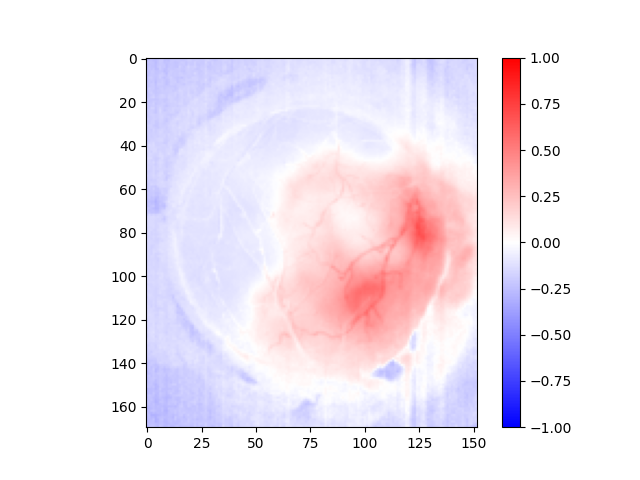
\includegraphics[scale=0.4]{m219_r25_t1/avg_strf}
	\caption{The figure shows the average activation over time of each pixel in the recording. Two regions can be identified as having the strongest activity.}
	\label{fig:strf_m219_r25}
\end{figure}

\begin{figure}
\centering
\animategraphics[width=0.7\linewidth,controls]{30}{m219_r25_t1/video/image}{1}{31}
\caption{This figure is generated using the same data as Figure \ref{fig:strf_m219_r25} but instead the STRF of each neuron is only summed accross the spatial dimension, resulting in a video where the average STRF value is shown for each moment $t$. This recording is also available in the github repository.}
\end{figure}

\begin{figure}
	\begin{subfigure}{0.45\textwidth}
	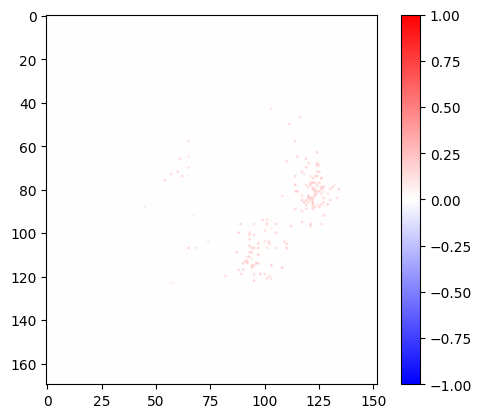
\includegraphics[width=\textwidth]{50_trials}
	\caption{This panel shows the correlation between the actual and predicted response. This network was trained on 40 trials, and 10 trials were used for testing. The scores (i.e correlations) were then averaged for each pixel and plotted here.}
	\end{subfigure}
	\hfill
	\begin{subfigure}{0.45\textwidth}
	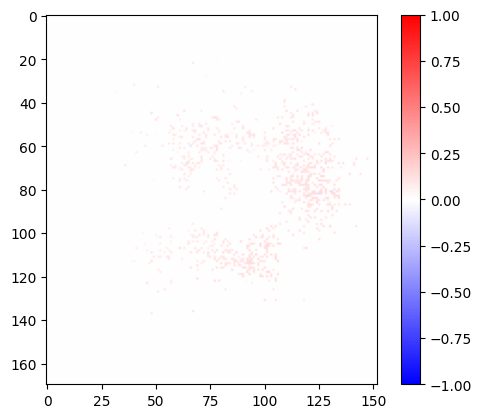
\includegraphics[width=\textwidth]{90_trials}
	\caption{The same procedure as in the left panel was applied here. In this case, 72 trials were used for training and 18 for testing. There are significantly more correlations visible in the figure, probably due to the increased amount of input data.}
\end{subfigure}
	\caption{The figure shows the average Pearson correlation scores per pixel between the actual response to the stimulus and the response predicted by the DSTRF. A comparison is made between models trained on varying amounts of data.}
	\label{fig:50trials}
\end{figure}

